%----------------------------------------------------------------------------------------
%	PACKAGES AND THEMES
%----------------------------------------------------------------------------------------
\PassOptionsToPackage{table}{xcolor}
\documentclass[aspectratio=169,xcolor=dvipsnames,svgnames,x11names,fleqn]{beamer}
% \documentclass[aspectratio=169,xcolor=dvipsnames,fleqn]{beamer}

\usetheme{RedVelvet}

\usefonttheme[onlymath]{serif}
\newcommand{\showanswers}{yes}


\usepackage{xspace}
\usepackage{amsmath}
\usepackage{amssymb}
\usepackage{amsfonts}
\usepackage{color}
\usepackage{physics}
% \usepackage{mathbb}
\usepackage{rahul_math}
\usepackage{bigints}

\usepackage{graphicx} % Allows including images
\usepackage{booktabs} % Allows the use of \toprule, \midrule and \bottomrule in tables
\usepackage{tikz,pgfplots}

\usepackage{subfigure}
\usetikzlibrary{arrows}
\usepackage{minted}
\definecolor{LightGray}{gray}{0.9}
\definecolor{cream}{rgb}{0.92, 0.9, 0.55}
\definecolor{lightblue}{rgb}{0.68, 0.85, 0.9}


\usepackage{xcolor-material}
\usetikzlibrary{fit}
\usetikzlibrary{matrix}
\tikzset{%
apple/.pic={
    \fill [MaterialBrown] (-1/8,0)  arc (180:120:1 and 3/2) coordinate [pos=3/5] (@)-- ++(1/6,-1/7)  arc (120:180:5/4 and 3/2) -- cycle;
    \fill [MaterialLightGreen500] (0,-9/10)  .. controls ++(180:1/8) and ++(  0:1/4) .. (-1/3,  -1) .. controls ++(180:1/3) and ++(270:1/2) .. (  -1,   0) .. controls ++( 90:1/3) and ++(180:1/3) .. (-1/2, 3/4) .. controls ++(  0:1/8) and ++(135:1/8) .. (   0, 4/7)
    }
    }

\newcommand{\leftdoublequote}{\textcolor{blue}{\scalebox{3}{``}}}

\newcommand{\rightdoublequote}{\textcolor{blue}{\scalebox{3}{''}}}


\usepackage{textcomp}
\usepackage{fontawesome}
\usepackage{tikz,pgfplots}
\usetikzlibrary{shapes.callouts}
\usetikzlibrary{arrows}


\usepackage{overpic}

%----------------------------------------------------------------------------------------
%	TITLE PAGE
%----------------------------------------------------------------------------------------

\usepackage{tikz-qtree,tikz-qtree-compat}
\usetikzlibrary{tikzmark}
\usetikzlibrary{calc}


\title[CPE 486/586: Machine Learning]{CPE 486/586: Machine Learning for Engineers} % The short title appears at the bottom of every slide, the full title is only on the title page
\subtitle{11 Unsupervised Learning: Clustering}

\author[Rahul Bhadani] {{\Large \textbf{Rahul Bhadani}}}

\institute[UAH] % Your institution as it will appear on the bottom of every slide, maybe shorthand to save space
{
    Electrical \& Computer Engineering,  The University of Alabama in Huntsville
}
\date

% \titlegraphic{
%    \includegraphics[width=0.4\linewidth]{figures/UAH_primary.png}
% }

\begin{document}

%-------------------------------------------------
\begin{frame}
    \titlepage
\end{frame}

%-------------------------------------------------
\begin{frame}{Outline}
    \backgroundtableofcontents
\end{frame}





\begin{sectionframe}{\faLightbulb}{Motivation}
\end{sectionframe}

\begin{frame}{What is Unsupervised Learning?}
    \begin{itemize}
    \item In contrary to supervised learning, in unsupervised learning, there is no labeled data.
    \item That is to say, there is no human-supervision involved in labeling a feature vector.
\end{itemize}
\end{frame}

\begin{frame}{When to use Unsupervised Learning?}
\begin{enumerate}
    \item When we are not sure what we are looking at, unsupervised learning is a useful technique.
    \item When we want to just group together several things but we don't care about what these groups belong to.
    \item To find a hidden pattern.
\end{enumerate}
\end{frame}

\begin{frame}{When Unsupervised Learning is Useful?}
    \begin{enumerate}
\item Market segmentation: finding relationships between customer variables so that a company can plan its marketing and choose which customer segments to target.
\item Image grouping: splitting a data set of cat and dog photographs into two groups.
\item Image segmentation: dividing an image into regions of similar color or texture.
\item Biological taxonomy (next slide).
    \end{enumerate}
    \end{frame}

    \begin{frame}{Example: Biology Taxonomy}
        \begin{center}
            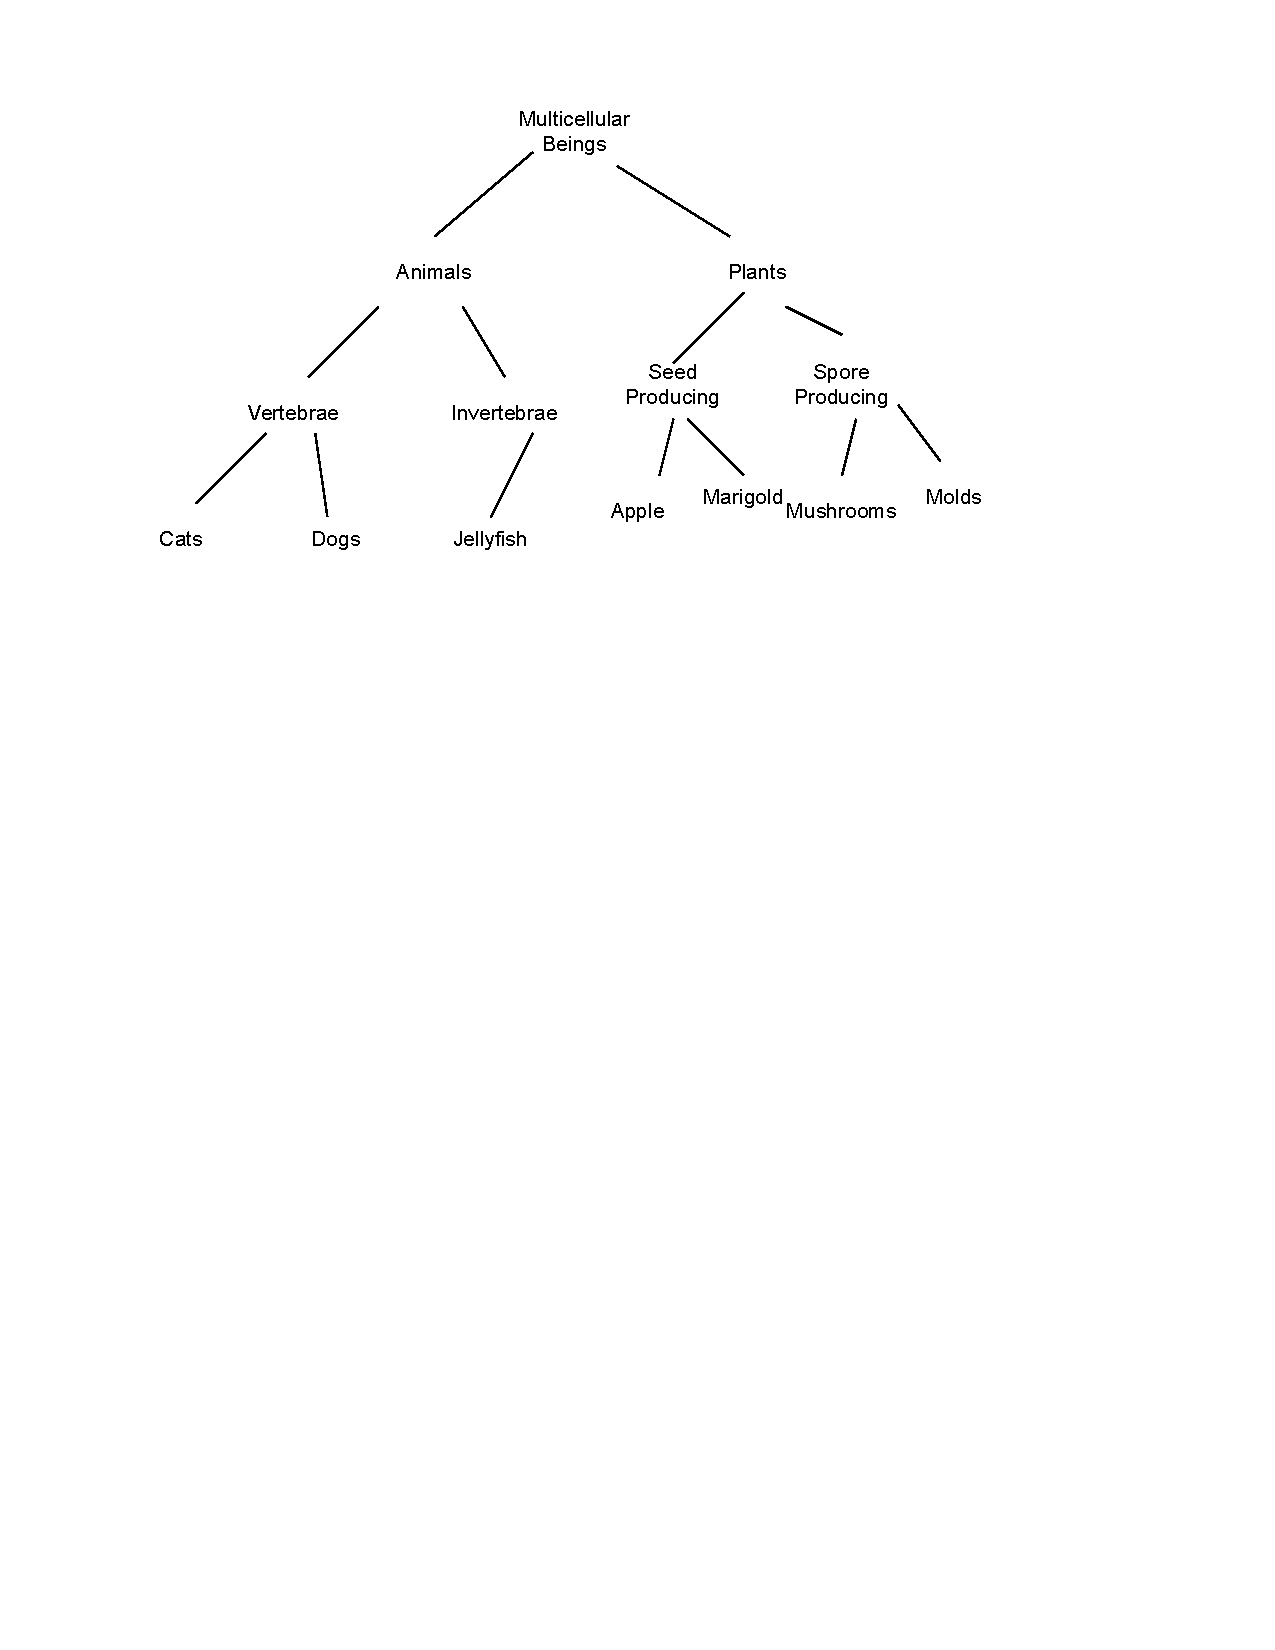
\includegraphics[width=1.0\textwidth]{figures/Taxonomy.pdf}
        \end{center}
    \end{frame}

    \begin{sectionframe}{\faBraille}{Clustering}
    \end{sectionframe}
    

    \begin{frame}{Clustering}
            \begin{itemize}
            \item Clustering is a type of unsupervised learning aimed at dividing unlabeled data into various groups.
            \item Clustering places points with similar features in the same group and points with dissimilar features in different groups.
\item Clustering appears in market segmentation, outlier detection, network analysis and the applications listed earlier.
            \end{itemize}
    \end{frame}
        

    \begin{frame}{Types of Clustering}
        \begin{enumerate}
            \item Centroid-based or Partition-based clustering
            \begin{itemize}
                \item Example: K-means
            \end{itemize}
            \item Connectivity-based clustering
            \begin{itemize}
                \item Example: Hierarchical clustering
            \end{itemize}
            \item Density-based clustering
            \begin{itemize}
                \item Example: DBSCAN
            \end{itemize}
            \item Graph-based clustering
            \begin{itemize}
                \item Example: Affinity Propagation
            \end{itemize}
            \item Distribution-based Clustering
            \begin{itemize}
                \item Example: Gaussian Mixture-Models
            \end{itemize}
        \end{enumerate}
    \end{frame}

    \begin{frame}{K-Means}
    \begin{itemize}
\item K-means is the most common clustering method. It is a heuristic that seeks to minimize the within-cluster sum of squared distances to the centroids.
\item It starts by assuming the number of clusters, $K$.
\item With $K$ clusters, we start by initializing $K$ centroids.
        \item Consider the following data points in two clusters:
        \begin{itemize}
            \item Cluster 1: (1,1), (2,1), (1,2), (2,2), (3,1)
            \item Cluster 2: (5,5), (5,6), (6,5), (6,6), (7,5), (6,7)
        \end{itemize}
    \end{itemize}
    \end{frame}

    \begin{frame}{K-Means Clustering Example}
        \begin{itemize}
           \item \textbf{Step 1:} Initialize two centroids. Here we pick the data points (1,1) and (5,5).
            \begin{center}
            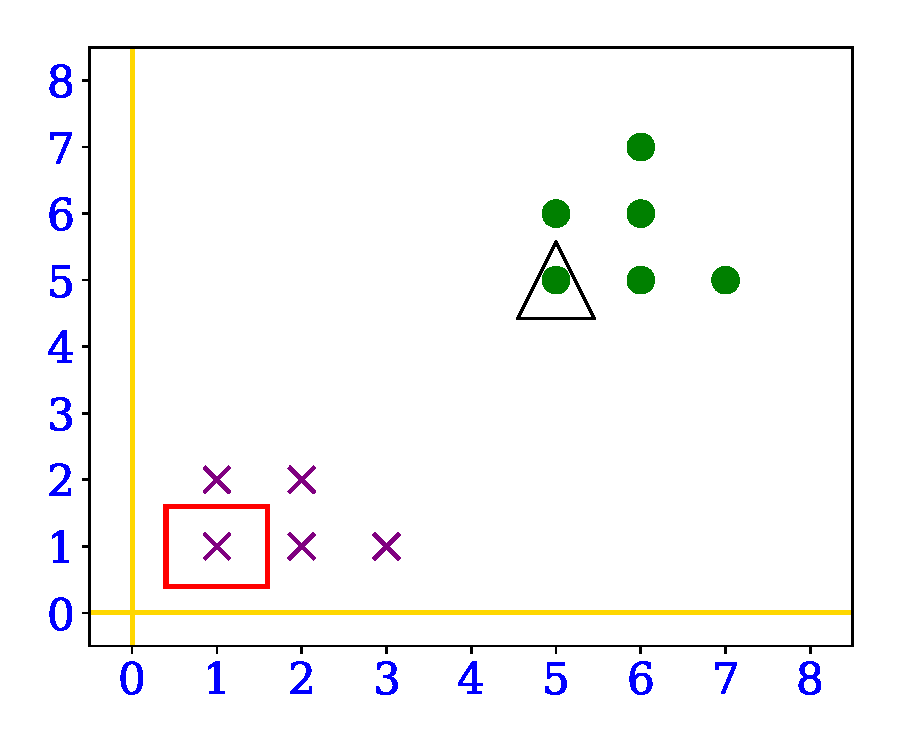
\includegraphics[width=0.44\textwidth]{figures/two_clusters.pdf} % Replace kmeans_step1.png with your image
            \end{center}
        \end{itemize}
    \end{frame}

    \begin{frame}{K-Means Clustering Example (Continued)}
        \begin{itemize}
        \item \textbf{Step 2:} Calculate Euclidean distance of each point to the centroid and assign each data point to the nearest centroid.
        \item In this case, it is clear to see that data points closer to (1,1) are (1,1), (2,1), (3,1), (1,2), (2,2) and data points closer to (5,5) are (5,5), (5,6), (6,5), (6,6), (7,5), and (6,7).
        \item Now, we recalculate two centroids $(x_1, y_1)$ and $(x_2, y_2)$.
        \begin{multiequation}
        x_1 &= \frac{1+2+3+1+2}{5} = \frac{9}{5} = 1.8 \\
        y_1 &= \frac{1+1+1+2+2}{5} = \frac{7}{5} = 1.4 \\
        x_2 &= \frac{5+5+6+6+7+6}{6} = \frac{35}{6} = 5.83\\
        y_2 &= \frac{5+6+5+6+5+7}{6} = \frac{34}{6} = 5.66
        \end{multiequation}
    \end{itemize}
    \end{frame}
    
    \begin{frame}{K-Means Iteration}
    \begin{itemize}
        \item Hence, the new centroids are (1.8, 1.4) and (5.83, 5.66).
       \item Next, we reassign the points by computing their distances to the two new centroids.
\item If a point is $(x_i, y_i)$ and the two centroids are $(x_{c1}, y_{c1})$ and $(x_{c2}, y_{c2})$, then:
        \begin{itemize}
        \item If $\sqrt{(x_i - x_{c1})^2 + (y_i - y_{c1})^2} < \sqrt{(x_i - x_{c2})^2 + (y_i - y_{c2})^2}$, then $(x_i, y_i)$ belongs to cluster 1.
        \item Otherwise, it belongs to cluster 2.
        \item With the new centroids, the assignments stay the same, so K-means stops after this pass.
        \end{itemize}
    \end{itemize}
    \end{frame}

    \begin{frame}{K-Means Convergence}
        \begin{itemize}
            \item We repeat the assignment and update steps until the assignments stop changing. The result is a local minimum of the within-cluster sum of squares, so a different initialization can give a different answer.
\item For $K$ clusters, point $(x_i, y_i)$ goes to cluster $c_i = \arg\min_{j} \left( (x_i - x_{cj})^2 + (y_i - y_{cj})^2 \right)$.
        \end{itemize}
    \end{frame}
        
    \begin{frame}{Hierarchical Clustering}
        \begin{itemize}
            \item Used to group similar objects.
            \item We don't need a pre-determined number of clusters.
            \item There are two types of hierarchical clustering:
            \begin{enumerate}
                \item Agglomerative clustering
                \item Divisive hierarchical clustering
            \end{enumerate}
        \end{itemize}
    \end{frame}

    \begin{frame}{Agglomerative Clustering}
        \begin{itemize}
           \item The algorithm starts with one cluster per data point and repeatedly merges the two closest clusters.
\item A linkage rule defines the distance between two clusters: single (closest pair of points), complete (farthest pair), average, or Ward (smallest increase in within-cluster variance).
            \item Usually agglomerative clustering is presented as a dendrogram.
        \end{itemize}
        \begin{center}
            % \includegraphics[width=0.8\textwidth]{agglomerative_clustering.png} % Replace agglomerative_clustering.png with your image
        \end{center}
    \end{frame}

    \begin{frame}{Agglomerative Clustering (Continued)}
        \begin{itemize}
        \item Then we can cut the dendrogram at any point to get the desired number of clusters.
    \end{itemize}
    \begin{center}
        % \includegraphics[width=0.8\textwidth]{dendrogram_cut.png} % Replace dendrogram_cut.png with your image
    \end{center}
\end{frame}

\begin{frame}{Divisive Hierarchical Clustering}
\begin{itemize}
\item We start with one cluster that holds the whole data set and split it repeatedly until no cluster holds more than one point.
\item The dendrogram shows the merge or split order in two dimensions, whatever the number of features.
\item Agglomerative clustering stores an $n \times n$ distance matrix, so it suits modest sample sizes.
\end{itemize}
\end{frame}

\begin{frame}{Density-based Clustering}
    \begin{itemize}
    \item Density-based methods group points that lie in dense regions. Density is measured by counting the neighbors within a distance $\varepsilon$.
\item These methods find regions where points are concentrated and treat sparse or empty regions as gaps between clusters. Points outside the clusters are labeled as noise.
\end{itemize}
\end{frame}

\begin{frame}{Density-based Spatial Clustering of Applications with Noise (DBSCAN)}
\begin{itemize}
   \item The DBSCAN algorithm groups points that lie in dense regions. Regions of low density separate the clusters.
\item DBSCAN uses a specified distance to separate dense clusters from sparser noise. With a spatial index and a small $\varepsilon$, it runs in about $O(n \log n)$ time. Its worst case is $O(n^2)$.
\end{itemize}
\end{frame}

\begin{frame}{DBSCAN Limitations and Example}
    \begin{columns}
        \column{0.4\linewidth}
        \begin{itemize}
           \item DBSCAN works well only when one search distance $\varepsilon$ suits the clusters. That requires the meaningful clusters to have similar densities.

        \end{itemize}
        \begin{itemize}
           \item By eye, the clusters are easy to see. K-means still assigns the outliers to a cluster, and they pull the centroids toward them.
        \end{itemize}
        \column{0.6\linewidth}
        \begin{center}
            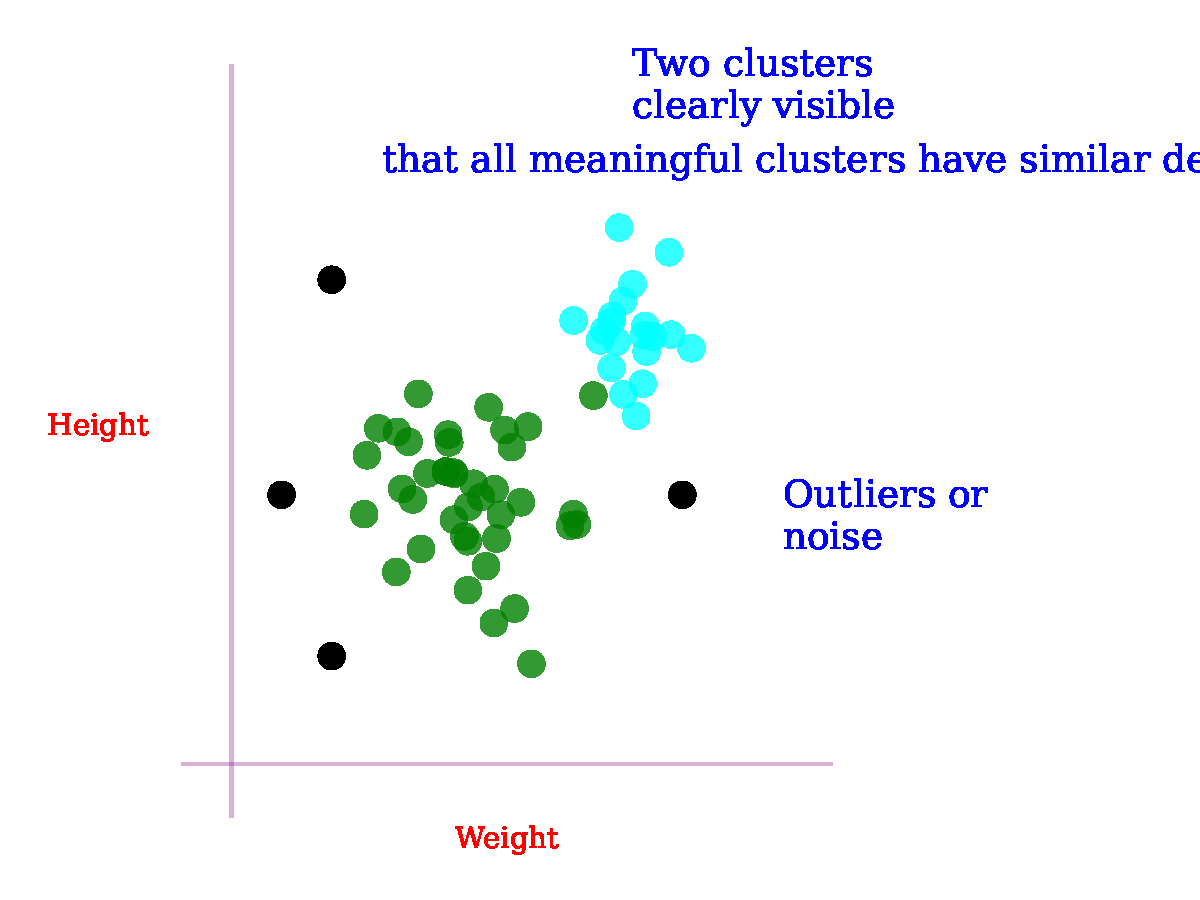
\includegraphics[width=1.0\textwidth]{figures/two_clusters_with_outliers.pdf} % Replace dbscan_example.png with your image
        \end{center}
    \end{columns}
    
\end{frame}

\begin{frame}{Points to Consider While Applying DBSCAN}
    \begin{itemize}
   \item Clusters form high-density regions.
\item Noise points are sparse and lie away from the dense regions.
\end{itemize}
\end{frame}

\begin{frame}{Let's Start with Unclustered Data}
%     \begin{center}
%     \includegraphics[width=0.8\textwidth]{unclustered_data.png} % Replace unclustered_data.png with your image
% \end{center}
\end{frame}

\begin{frame}{DBSCAN - Step 1: Count Close Points}
    \textbf{Step 1:} Count the number of points close to each point.
\vfill
\end{frame}

\begin{frame}{DBSCAN - Step 1: Count Close Points}
    \begin{itemize}
    \item We start with the red point and draw an orange circle around it.
  \item The orange circle contains 8 other points.
\item So the red point has 8 neighbors.
\item Note: The radius of the circle, $\varepsilon$ (eps), is a user-defined parameter.
\item Repeating this for another red point, we find 5 neighbors.
\item  The green point is not close to any other point.
\item A core point has at least 4 neighbors within $\varepsilon$. This threshold, minPts, is a second user-defined parameter.
\end{itemize}
\begin{center}
    % \includegraphics[width=0.8\textwidth]{dbscan_step1_count.png} % Replace dbscan_step1_count.png with your image
\end{center}
\end{frame}

\begin{frame}{DBSCAN - Defining Core and Non-Core Points}
    \begin{itemize}
    \item \item Points with at least 4 neighbors are core points (red). The remaining points are non-core points (green).
\end{itemize}
\vfill
\end{frame}

\begin{frame}{}
\end{frame}


\begin{frame}{DBSCAN - Building the First Cluster}
    \begin{itemize}
\item We pick a core point at random and assign it to the first cluster.
\item Core points within $\varepsilon$ of that point join the first cluster.
\item Core points within $\varepsilon$ of the growing cluster join it in turn.
\item When no further core point can join, we add the non-core points that lie within $\varepsilon$ of a core point in the cluster. These border points join the cluster without extending it.
\item This completes the first cluster.
\end{itemize}
\end{frame}

\begin{frame}{DBSCAN - Building Subsequent Clusters}
    \begin{itemize}
    \item Now we look at other core points that are not part of the first cluster and repeat the process to get the second cluster.
    \item Non-core points with no core point within $\varepsilon$ are labeled noise.
\end{itemize}
\end{frame}

\begin{frame}{Graph-based Clustering}
    \begin{itemize}
  \item Graph-based methods treat the data as a graph, with points as nodes and pairwise similarities as edge weights. They split the graph into groups of strongly connected nodes. Spectral clustering is the standard example.
\end{itemize}
\end{frame}


\begin{frame}{Affinity Propagation Clustering}
    \begin{itemize}
\item Affinity propagation chooses the number of clusters itself. A user-set preference, placed on the diagonal $S(k,k)$, controls how many exemplars emerge.
\item In simple terms, a data point sends messages to the other points. A message informs the target of its relative attractiveness to the sender.
    \item Each target then responds to all senders with a reply informing each sender of its availability to associate with the sender, given the attractiveness of the messages that it has received from all other senders.
\end{itemize}
\end{frame}

\begin{frame}{Affinity Propagation Details}
    \begin{itemize}
    \item Senders reply to the targets with messages informing each target of the target's revised relative attractiveness to the sender, given the availability messages it has received from all the targets.
    \item The message-passing procedure is repeated until a consensus is achieved.
    \item Once the sender is associated with one of its targets, that target becomes the point's exemplar.
    \item All points with the same exemplar are placed in the same cluster.
\item Note: The similarity $S(i,k)$ is the input to the algorithm. A common choice is the negative squared Euclidean distance. The attractiveness messages above are the responsibilities $R(i,k)$.
\end{itemize}
\end{frame}

\begin{frame}{Affinity Propagation Example}
    \begin{itemize}
    \item Example: (1,2) and (3,4)
   \item $-\left[(1-3)^2 + (2-4)^2\right] = -8$ is the similarity score between (1,2) and (3,4).
\end{itemize}
\end{frame}

\begin{frame}{Affinity Propagation Algorithm}
    \begin{enumerate}
       \item Calculate the similarity matrix $S$ over pairs of points, say the negative squared Euclidean distance. Set the diagonal $S(k,k)$ to the preference, for example the median of the similarities.
        
        \vspace{0.5em}
        $\begin{array}{c|ccc c}
        & A1 & A2 & A3 & \cdots \\
        \hline
        A1 & \square & \square & \square & \square \\
        A2 & \square & \square & \square & \square \\
        A3 & \square & \square & \square & \square \\
        \vdots & \square & \square & \square & \square
        \end{array}$
        
    \end{enumerate}
    \end{frame}


\begin{frame}{Affinity Propagation Algorithm}

    \begin{enumerate}
        \item[2.] Calculate the Responsibility Matrix:
        \begin{itemize}
           \item Initialize the availability matrix $A$ and the responsibility matrix $R$ with zeros.
\item Update $R$ iteratively using the formula:
$$R(i, k) = S(i, k) - \max_{k' \neq k} \{ A(i, k') + S(i, k') \}$$
        \end{itemize}

    \end{enumerate}

\end{frame}

\begin{frame}{Affinity Propagation Algorithm}

    \begin{enumerate}
\item[3.] Then, we calculate the availability matrix. For $i \neq k$:
\[
    A(i, k) = \min \left( 0, R(k, k) + \sum_{\substack{i' \neq i \\ i' \neq k}} \max(0, R(i', k)) \right)
\]
and on the diagonal:
\[
    A(k, k) = \sum_{i' \neq k} \max(0, R(i', k))
\]
\item[4.] Exemplars (Cluster Centers): point $k$ is an exemplar when $A(k,k) + R(k,k) > 0$.
\item[5.] Once we have exemplars, assign a data point to its most similar exemplar. Points that share an exemplar form one cluster.


    \end{enumerate}

\end{frame}

\begin{frame}{Distribution-based Clustering}
    \begin{figure}
        \centering
        \begin{minipage}[b]{0.45\textwidth} % Left column for the figure
            \centering
            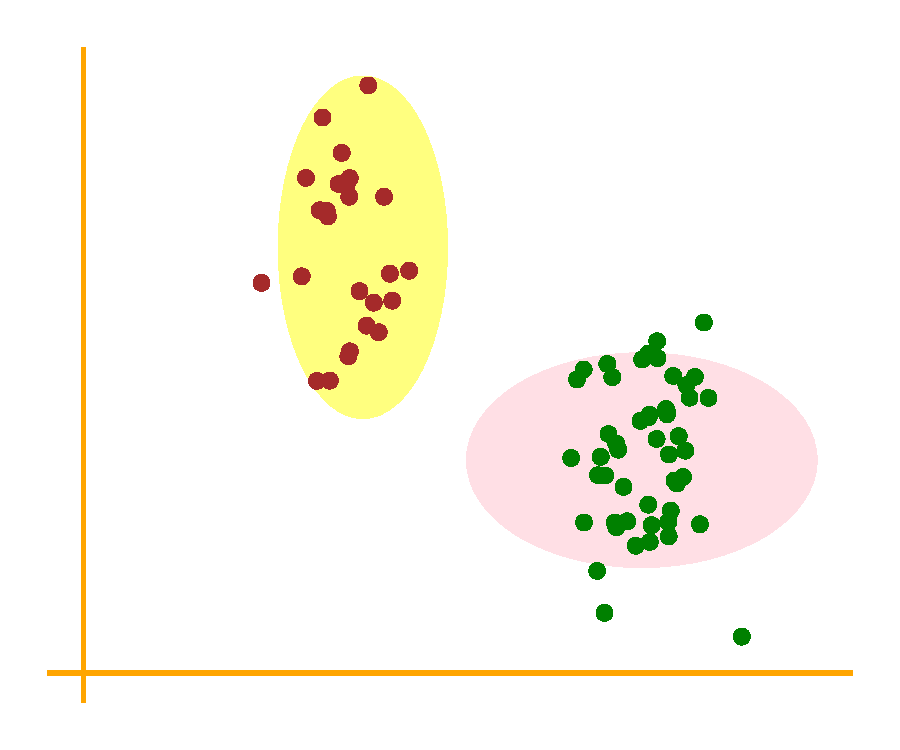
\includegraphics[width=\textwidth]{figures/distribution_based_clustering.pdf} % Replace with your image
        \end{minipage}
        \hfill
        \begin{minipage}[b]{0.45\textwidth} % Right column for the text
            \begin{itemize}
                \item Distribution-based methods group data points together based on their likelihood of belonging to the same probability distribution.
            \end{itemize}
        \end{minipage}
    \end{figure}
\end{frame}

\begin{frame}{Distribution-based Clustering - Notes}
    \begin{itemize}
   \item Distribution-based methods use statistical inference to cluster data. The closer a point lies to a component's center, the higher its probability of assignment to that component.
\item Distribution-based methods can fit cluster shapes, such as elongated ellipses, that K-means misses. This works when the clusters follow the assumed distribution.
\item A Gaussian mixture overfits when it has too many components, or full covariance matrices with too little data. A component can also collapse onto a single point, which drives its variance to zero and the likelihood to infinity.
\end{itemize}
\end{frame}

\begin{frame}{Gaussian Mixture Model (GMM)}
    \begin{itemize}
    \item GMM assumes the data come from a mixture of $K$ Gaussian distributions with unknown parameters. A point is drawn from one component, chosen with probability equal to that component's mixing weight. The Expectation-Maximization (EM) algorithm fits the parameters.
\item The parameters start at random values. In the E-step, the current parameters give the probability that a point belongs to a given component.
\item In the M-step, the component parameters are re-estimated from the data, with points weighted by those probabilities.
\end{itemize}
\end{frame}

\begin{frame}{Gaussian Mixture Model - E-Step}
    \begin{enumerate}
    \item E-Step:
    \begin{enumerate}
        \item Compute the probability that each data point belongs to each Gaussian component.
        \item Then soft-assign a point to clusters, that is, a point $\xbf$ belongs to cluster 1 with 60\% probability, to cluster 2 with 30\% probability and to cluster 3 with 10\% probability (just an example).
\item The probability that point $\xbf_i$ belongs to component $k$ is
\[
    \gamma_{ik} = \frac{\pi_k\,\mathcal{N}(\xbf_i \mid \boldsymbol{\mu}_k, \boldsymbol{\Sigma}_k)}{\sum_{j=1}^{K} \pi_j\,\mathcal{N}(\xbf_i \mid \boldsymbol{\mu}_j, \boldsymbol{\Sigma}_j)}
\]

    \end{enumerate}
\end{enumerate}
\end{frame}

\begin{frame}{Gaussian Mixture Model - M-Step}
    \begin{enumerate}
    \setcounter{enumi}{1}
    \item M-Step:
    \begin{enumerate}
        \item Update the parameters of each Gaussian component based on the soft assignments.
       \item Recalculate parameters of Gaussian components such as mean, variance, and weights.

    \end{enumerate}
\item The two steps repeat until the log-likelihood rises by less than a set tolerance.\end{enumerate}
\end{frame}

\begin{sectionframe}{\faBroom}{Evaluating Cluster Quality}
\end{sectionframe}


\begin{frame}{Evaluating Cluster Quality -- Extrinsic Measure}
    \begin{enumerate}
    \item Extrinsic Measure: Requires ground truth labels.
    \begin{enumerate}
        \item Rand Index
        \item Mutual Information
        \item V-measure
        \item Fowlkes-Mallows Scores
    \end{enumerate}
\end{enumerate}
\end{frame}

\begin{frame}{Evaluating Cluster Quality - Rand Index}
    \begin{enumerate}
    \item Rand Index:
    \begin{itemize}
       \item Measures the similarity between the predicted and true cluster assignments through pairwise comparisons. A pair counts as correct when both assignments place it in the same cluster, or both place it in different clusters.

        \item Higher Rand Index means higher similarity.
        \item \[RI = \frac{\text{\# pairwise correct predictions}}{\text{Total \# possible pairs}}\]
       \item The Adjusted Rand Index corrects for agreement between two clusterings that occurs by chance.
    \end{itemize}
\end{enumerate}
\end{frame}

\begin{frame}{Evaluating Cluster Quality - Mutual Information, V-measure, Fowlkes-Mallows Scores}
\begin{enumerate}
    \setcounter{enumi}{1}
    \item Mutual Information: The degree of agreement between clusters is computed by joint and marginal probabilities.
    \item V-measure: Measures the correctness of cluster assignments using conditional entropy analysis.
    \item Fowlkes-Mallows Scores: Measures the correctness of the cluster assignments using pairwise precision and recall. A higher score signifies higher correctness.
\end{enumerate}
\end{frame}

\begin{frame}{Evaluating Cluster Quality -- Intrinsic Measures}
\begin{enumerate}
    \setcounter{enumi}{1}
    \item Intrinsic Measure: Doesn't require ground truth labels.
    \begin{enumerate}
        \item Silhouette Coefficients: Measures the between-cluster distance against within-cluster distance. A higher score signifies better-defined clusters.
        \item Calinski-Harabasz Index: Measures the between-cluster dispersion against within-cluster dispersion.
        \item Davies-Bouldin Index: Measures the size of clusters against the average distance between clusters. A lower score signifies better-defined clusters.
    \end{enumerate}
\end{enumerate}
\end{frame}

\begin{frame}{Cluster Quality Evaluation Formulas}
    \begin{itemize}
    \item \textbf{1. ARI (Adjusted Rand Index)}
    \begin{itemize}
       \item $\text{Expected index} = \frac{\text{\# pairs in the same cluster (actual)} \times \text{\# pairs in the same cluster (predicted)}}{\text{Total no. of possible pairs}}$
\item $ARI = \frac{\text{\# pairs in the same cluster in both} - \text{Expected index}}{\text{Average \# pairs in same cluster for actual and predicted} - \text{Expected index}}$
    \end{itemize}
    
\end{itemize}
\end{frame}

\begin{frame}{Cluster Quality Evaluation Formulas (Continued)}
    \begin{itemize}
    \item \textbf{2. Mutual Information (MI)}
    \begin{itemize}
        \item Adjusted MI (AMI)
        \item Normalized MI (NMI)
        \item $P(i, j) = \text{Probability of data in cluster } i \text{ (actual) and cluster } j \text{ (predicted)}$
        \item $P(i) = \text{Probability of data in cluster } i \text{ (actual)}$
        \item $P'(j) = \text{Probability of data in cluster } j \text{ (predicted)}$
       \item $H(U) = \text{Entropy of actual cluster assignment} = -\sum_{i \in U} P(i) \log P(i)$, where $U$ is the set of actual clusters
\item $H(V) = -\sum_{j \in V} P'(j) \log P'(j)$, where $V$ is the set of predicted clusters
        \item $MI = \sum_{i \in U} \sum_{j \in V} P(i, j) \log \frac{P(i, j)}{P(i) P'(j)}$
        \item $NMI = \frac{MI}{\frac{1}{2} [H(U) + H(V)]}$
        \item $AMI = \frac{MI - E[MI]}{\frac{1}{2} [H(U) + H(V)] - E[MI]}$
    \end{itemize}
\end{itemize}
\end{frame}

\begin{frame}{Cluster Quality Evaluation Formulas (Continued)}
    \begin{itemize}
    \item \textbf{3. V-Measure}
    \begin{itemize}
\item $H(C|K) = $ conditional entropy of the true classes $C$ given the cluster assignments $K$
\item $H(C|K) = -\sum_{c}\sum_{k} \cfrac{n_{ck}}{n} \log \left( \cfrac{n_{ck}}{n_k} \right)$, where $\cfrac{n_{ck}}{n_k} = \cfrac{\text{no. of samples labelled } c \text{ in cluster } k}{\text{Total no. of samples in cluster } k}$
\item $H(C) = -\sum_{c} \cfrac{n_c}{n} \log \left( \cfrac{n_c}{n} \right)$
\item $\text{Homogeneity}(h) = 1 - \cfrac{H(C|K)}{H(C)}$
        \item $H(C|K) = -\sum_{k} n_{ck} \log \left( \cfrac{n_{ck}}{n_k} \right) \rightarrow \frac{\text{no. of samples labelled C in cluster k}}{\text{Total no. of samples in cluster k}}$
        \item $\text{Completeness}(c) = 1 - \cfrac{H(K|C)}{H(K)}$
        \item $V \text{ measure} = \cfrac{2 \cdot h \cdot c}{h + c}$
    \end{itemize}
\end{itemize}
\end{frame}


\begin{frame}{Cluster Quality Evaluation Formulas (Continued)}
    \begin{itemize}

    \item \textbf{4. Fowlkes-Mallows Scores}
    \begin{itemize}
        \item $FMI = \frac{TP}{\sqrt{(TP + FP) \times (TP + FN)}}$
       \item $TP \rightarrow$ pairs in the same cluster in both the true and predicted assignments
\item $FP \rightarrow$ pairs in the same cluster in the prediction only
\item $FN \rightarrow$ pairs in the same cluster in the truth only
    \end{itemize}
    \item \textbf{5. Silhouette Coefficient (S)}
    \begin{itemize}
        \item $a = \text{Average distance between sample and all other points in the same cluster}$
        \item $b = \text{Average distance between sample and the points in the nearest other cluster}$
\item $s = \frac{b - a}{\max(a, b)}$ for one sample. The silhouette coefficient $S$ is the mean of $s$ over the samples.
    \end{itemize}
\end{itemize}
\end{frame}

\begin{frame}{Cluster Quality Evaluation Formulas (Continued)}
\begin{itemize}
    \item \textbf{6. Calinski-Harabasz Index}
    \begin{itemize}
        \item $K = \text{no. of clusters}$
        \item $n_q = \text{no. of points in cluster } q$
        \item $C_q = \text{cluster center of cluster } q$
        \item $n_E = \text{no. of data points}$
        \item $C_E = \text{cluster center of all points}$
       \item $\text{Between-cluster dispersion, } B = \sum_{q=1}^{K} n_q (C_q - C_E) (C_q - C_E)^T$
\item $\text{Within-cluster dispersion, } W = \sum_{q=1}^{K} \sum_{x \in \text{cluster } q} (x - C_q) (x - C_q)^T$
\item $\text{Calinski-Harabasz Score } (s) = \frac{\operatorname{tr}(B)}{\operatorname{tr}(W)} \times \frac{n_E - K}{K - 1}$
    \end{itemize}
\end{itemize}
\end{frame}

\begin{frame}{Cluster Quality Evaluation Formulas (Continued)}
    \begin{itemize}
        \item \textbf{7. Davies-Bouldin Index}
    \begin{itemize}
        \item $K = \text{\# clusters}$
        \item $S_i = \text{Average distance between each point in cluster } i \text{ to cluster center } C_i$
        \item $d_{ij} = \text{distance between cluster centers } C_i \text{ and } C_j$
\item $\text{Similarity measure } R_{ij} = \frac{\text{Sum of within-cluster distances}}{\text{Between-cluster distance}} = \frac{S_i + S_j}{d_{ij}}$
\item $DB = \text{Average of maximum similarity measures} = \frac{1}{K} \sum_{i=1}^{K} \max_{j \neq i} (R_{ij})$
    \end{itemize}
\end{itemize}
\end{frame}
    
      %------------------------------------------------
    
    \begin{frame}[containsverbatim]{Python Notebook}
    \begin{center}
    \small
    { \color{Red}{\url{https://github.com/rahulbhadani/CPE486586_FA26/blob/master/Code/CPE486586_Ch11_Unsupervised_Learning.ipynb}}}
    \end{center}
    \end{frame}
    
    %------------------------------------------------
    
    \begin{frame}
        \Huge{\centerline{\color{MediumBlue}\textbf{The End}}}
    \end{frame}

\end{document}